\section{Motivation} \label{sec:moti}
As we know there are seven page types.
Among of them, segment descriptor pages are rarely updated, as they are almost const structures.  
However, the page-table pages are frequently changed from/to writable pages 
and these changes are driven by the process creations and exits.

Base on the above descriptions, we know that the page-type changes could trigger the invalidation of IOTLB entries.


From the above descriptions, we can summarize the dependency between the guest page table and the IOTLB flushing into two key points. We list them as follows:
\begin{enumerate}
\item (O1) Each page-type change (like the changes in Figure~\ref{fig:page-type-update}) will trigger the invalidation of at least one IOTLB entry.
\item (O2) The main source of causing IOTLB flushing is the page-type changes between writable pages and page-table pages.
\end{enumerate}

\begin{figure}[ht]
\centering
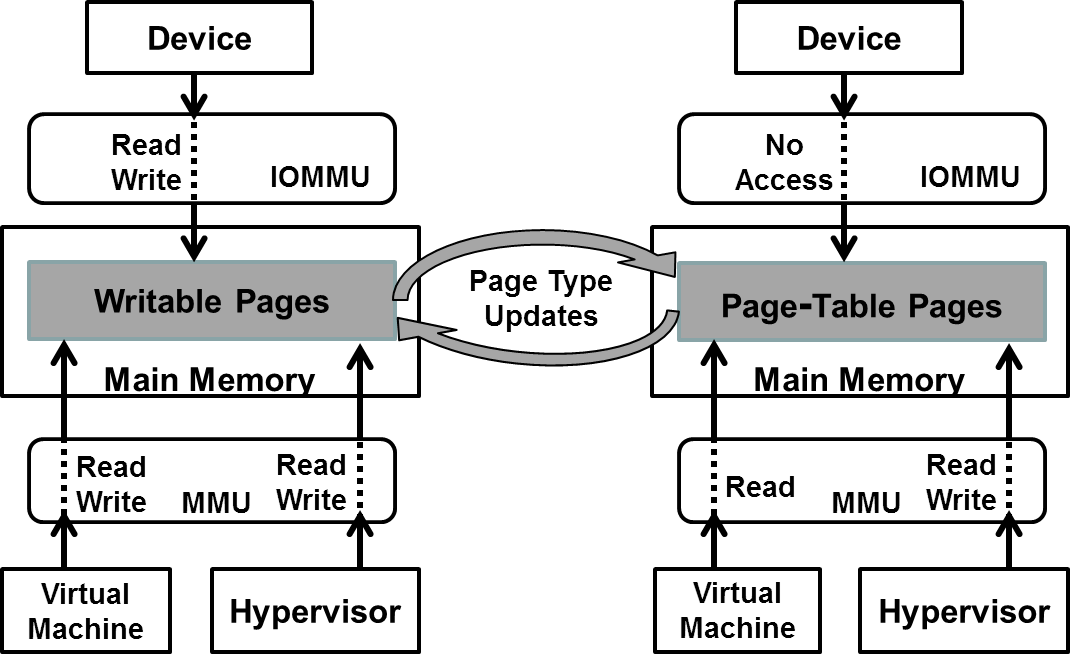
\includegraphics[width=0.5\textwidth]{image/background/wr2pt.png} \\
\caption{The page type updates between writable and page-table pages.}
\label{fig:wr2pt}
\end{figure}




Based on the observations, we are motivated to propose \name in order to reduce as many IOTLB flushes as possible for a maximum possible use of the IOTLB-path while retain the safety.
